\section{Decode-Time MBR Decoding}
\label{sec:decoding}

The frozen model still contains recoverable WER: at $G=128$ the oracle gap is 2.49~pp. Whether
decode-time methods can extract any of it — without touching parameters — is the question this
section answers. Training-time optimization, exhausted across two gradient estimators and two model types
(§4), provides no traction; the task at decode time is selecting among fixed outputs rather than adjusting the model
that generated them. The experimental program decomposed into two stages: first exhausting
CTC-internal information to determine where the acoustic model's discriminative capacity ends, then introducing external
language model posteriors to determine whether linguistic information bridges the gap.



\subsection{CTC-Internal Scoring: Exhaustion of the Acoustic Signal}
\label{sec:exhaustion}

Eleven CTC-internal and acoustic-feature-based scoring methods were applied to the LibriSpeech
dev-other N-best at $G$=16 (2864 utterances; greedy WER 6.0218\%; oracle WER 4.4418\%; oracle gap
1.58 pp). No method achieved statistically significant WER improvement over greedy. Table~\ref{tab:ctc-internal} reports representative results; Appendix~A.2 gives the full table with 95\% bootstrap confidence intervals for all thirteen methods.

\begin{table*}[t]
\centering
\caption{CTC-internal scoring methods at $G$=16, LibriSpeech dev-other.
Paired bootstrap, $B$=10\,000, seed=42 vs greedy. Seven additional CTC-internal strategies (argmax, length normalization, MBR-WER, MBR-CER at $\tau$=1, self-consistency, contrastive decoding, 14-feature MLP) all fell within $\pm$0.05~pp of greedy; see Appendix~A.2 for the full table.}
\label{tab:ctc-internal}
\begin{tabular}{lrrr}
\hline
Method & WER (\%) & $\Delta$ (pp) & $p$ \\
\hline
Greedy (baseline) & 6.022 & 0.000 & --- \\
MBR-CER ($\tau$=50, best CTC) & 5.987 & $-$0.035 & 0.163 \\
MC-dropout $T$=4 (5 seeds) & $6.030 \pm 0.020$ & $+$0.008 & 0/5 sig. \\
3-gram shallow fusion ($\alpha$=0.9) & 6.018 & $-$0.004 & 0.368 \\
Encoder value head & 6.020 & $-$0.002 & --- \\
\hline
\end{tabular}
\end{table*}

CTC posteriors at unit temperature are sharply peaked around the greedy output, so MBR degenerates to the mode of that distribution — which coincides with greedy by construction. The same mechanism explains why CTC-internal MBR with any temperature failed to reach significance: the information needed to separate oracle hypotheses from greedy-equivalent ones is not in the CTC posterior at all.

MC-dropout sampling showed no significant improvement across five seeds despite one initially promising seed that did not replicate (Appendix~C.1). Contrastive decoding degraded monotonically, consistent with CR-CTC's already-sharpened alignment distribution (Appendix~C.1). A trained 14-feature MLP rescorer achieved $R^2$=0.76 on in-distribution data but did not transfer to per-utterance ranking on dev-other (Appendix~C.1).

The encoder value head ablation trained an MLP on Zipformer-S encoder embeddings and ran a
three-way grid search over blending weights for CTC, value head, and RoBERTa PLL. The grid assigned
weight zero to the value head at the optimum: $\alpha$=0.6 CTC, $\beta$=0.0 value head, $\gamma$=0.4
RoBERTa. This result is consistent with the ranking-sufficiency property described in Proposition 2: CTC's
marginalization over alignments computes the sufficient statistic for hypothesis ranking, so the
residual variance in the raw encoder embeddings should carry no additional discriminative information
that a learned value function can extract. The zero encoder weight is consistent with the view that bypassing the marginalization exposes alignment-path noise rather than new acoustic signal.

The bottleneck lies between CTC and the linguistic domain, not within the acoustic model: every signal derivable from CTC posteriors, encoder features, or their combinations is exhausted, and any further improvement requires information the acoustic model does not have.



\subsection{External LM Rescoring with MBR}

Two pre-trained language models were introduced as external posterior sources: RoBERTa-base
\cite{liu2019roberta} evaluated via pseudo-log-likelihood (PLL) \cite{salazar2020pll}, and GPT-2
\cite{radford2019gpt2} evaluated via autoregressive log-likelihood. For a hypothesis
$y = y_1 \ldots y_n$, PLL is $\text{PLL}(y) = \sum_i \log P_{\text{RoBERTa}}(y_i \mid y_{\setminus
i})$, masking each token once and summing the resulting log-conditionals. Autoregressive LL is
$\text{LL}(y) = \sum_i \log P_{\text{GPT-2}}(y_i \mid y_{<i})$.

We use CER as the MBR loss rather than WER throughout. Using WER as both loss and evaluation metric on the same
candidate set is circular: optimising and measuring the same metric on the same population inflates
reported gains (we discuss the excluded MBR-WER result in Section~\ref{sec:cross_condition}). CER loss with WER evaluation is the fair comparison and is the
reported result in all tables.

\textbf{Ranking quality.} Per-utterance Spearman $\rho$ between scorer and candidate WER measures
discriminating power directly (more negative = better ranker). CTC
log-prob alone achieved $\rho$=$-$0.347. GPT-2 LL reached $\rho$=$-$0.401 (16\% stronger than CTC).
RoBERTa PLL reached $\rho$=$-$0.484 (39\% stronger than CTC). Linear interpolation of CTC and PLL at
$\alpha$=0.6 gave the peak $\rho$=$-$0.527 (52\% stronger than CTC). The interpolated peak lies outside
the PLL-alone 95\% CI upper bound ($-$0.475), confirming that the two information channels are
partially independent. RoBERTa PLL's bidirectional masking conditions on full sentence context; CTC's
posterior reflects frame-level acoustic probabilities only. The two sources therefore model
qualitatively different aspects of the hypothesis.

Utterance-length stratification makes the asymmetry sharper. On utterances with more than 20 words,
PLL $\rho$ reaches $-$0.561 while CTC $\rho$ falls to $-$0.316. Longer sequences give the language model
more context to exploit; CTC ranking quality degrades on the same sequences, possibly because length normalization disproportionately penalises longer candidate hypotheses. The
error-regime stratification is the most direct evidence for the information-bottleneck thesis. On the
665 recoverable utterances — those where greedy is suboptimal and a better hypothesis exists in the
N-best — CTC $\rho$ collapses to $-$0.241, a 36\% drop from the global $-$0.347. PLL $\rho$ holds at
$-$0.477 on the same 665 utterances, nearly unchanged from its global $-$0.484. The language model
maintains discriminating power exactly where the acoustic model loses it.

\textbf{Linear interpolation.} Argmax interpolation scored each candidate as
$\alpha \cdot \log P_{\text{CTC}} + (1-\alpha) \cdot \text{PLL}$ and selected the argmax. The
optimal $\alpha$=0.7 gave WER 5.92\% at $G$=16 ($\Delta$=$-$0.104 pp, $p$=0.0019, 95\% CI:
[$-$0.170, $-$0.039] pp), closing 6.5\% of the oracle gap. GPT-2 interpolation at $\alpha$=0.8 reached
5.99\% ($p$=0.024, 95\% CI: [$-$0.067, $-$0.002] pp), closing 2.1\%.
Three-gram shallow fusion at $\alpha$=0.9 produced 6.018\% ($p$=0.368): not statistically
significant. N-gram statistics do not carry the lexical-choice disambiguation
that RoBERTa PLL supplies from bidirectional context.

\textbf{MBR-CER with PLL posteriors.} MBR selects
$\hat{y} = \arg\min_{y_i} \sum_j w_j \cdot \text{CER}(y_i, y_j)$, where
$w_j \propto \exp(\text{PLL}_j / \tau)$, the temperature $\tau$ controlling posterior sharpness. At
$\tau$=1, WER is 7.93\% — 1.9 pp worse than greedy. The PLL posterior at unit temperature is as
sharply peaked as the CTC posterior; MBR collapses to the PLL argmax, which is not calibrated as an
acoustic ranker. At $\tau$=5, WER is 6.55\% — still above optimal. At $\tau$=10, WER drops to
5.79\% ($G$=16, $\Delta$=$-$0.232 pp, $p$<0.0001, 95\% CI: [$-$0.327, $-$0.138] pp), closing 14.7\% of
the oracle gap. This is more than twice the gain from linear interpolation at the same beam size.

The gap between MBR and interpolation has a mechanical explanation. Linear interpolation discards
all candidates except the one with the highest combined score — it is argmax with extra inputs. MBR
computes expected CER across all $G$ PLL-weighted candidates and picks the one that minimizes it.
Near-duplicate hypotheses, common at $G$=16 because k2 lattice paths cluster near the modal
transcript, each cast a weighted vote in the CER sum; MBR treats them as corroborating evidence.
A candidate that scores well in isolation but sits far from the cluster gets down-weighted.
Argmax has no such mechanism: it must commit to one winner regardless of what surrounds it.
This is why the MBR advantage grows with $G$ while interpolation plateaus.

At $G$=128, MBR-CER+PLL ($\tau$=10) achieved WER 5.53\% ($\Delta$=$-$0.493 pp, $p$<0.0001, 95\% CI:
[$-$0.586, $-$0.403] pp), closing 19.8\% of the $G$=128 oracle gap. Linear interpolation at $G$=128
peaked at 5.89\% — a gain of only 0.03 pp over its $G$=16 optimum. The two methods diverge
substantially as the candidate set grows. Section 5.3 examines the mechanism behind this divergence.

The 0.493 pp gain at $G$=128 conflates two contributions: \emph{(i)} adding PLL to the scoring
function, and \emph{(ii)} replacing argmax selection with MBR consensus. The best-$\alpha$
interpolation baseline (argmax rescoring with PLL+CTC, $\alpha$=0.8) achieves 5.89\% at $G$=128 —
a 0.13 pp reduction from greedy attributable to the PLL signal alone. MBR reduces this further to
5.53\%, an additional 0.36 pp attributable to consensus aggregation over the candidate set. The
MBR-specific contribution therefore accounts for approximately 73\% of the total $G$=128 gain. (Without CTC anchoring, pure PLL argmax degrades to 9.75\% WER — confirming that the two signals are complementary; the 0.13~pp attributed to PLL reflects its contribution \emph{within} the CTC-anchored ranking, not PLL operating in isolation.)

\subsection{Ranking Divergence Under Scaling: Why MBR Outperforms Interpolation}

\begin{figure*}[t]
  \centering
  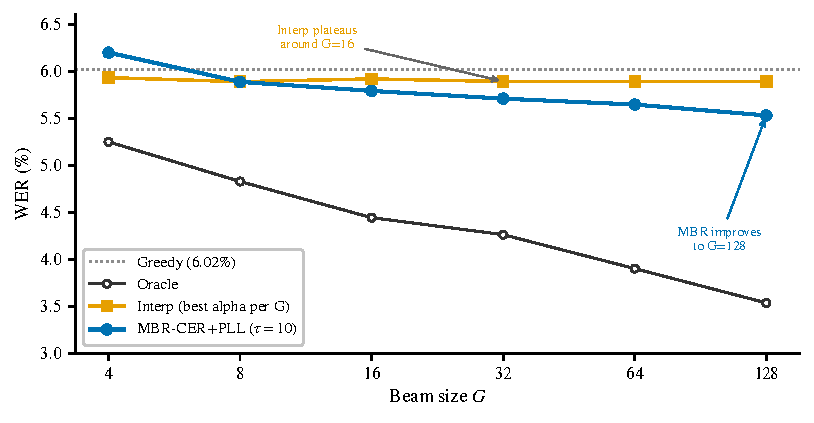
\includegraphics[width=\textwidth]{figures/fig4_g_scaling.pdf}
  \caption{WER vs beam size $G$ on dev-other. Interpolation (best $\alpha$ at each $G$) plateaus around $G=16$; MBR-CER+PLL ($\tau=10$) improves monotonically through $G=128$, closing 19.8\% of the oracle gap. See Fig.~\ref{fig:spearman} for the mechanistic explanation.}
  \label{fig:gscaling}
\end{figure*}

The beam-size scaling analysis fixes the candidate pool across $G$ to isolate the effect of
beam size; the oracle and Spearman-$\rho$ values along this curve are therefore internal to
the scaling sweep and are not expected to match the operational $G$=16/128 tables exactly.
Figure~\ref{fig:gscaling} shows WER as a function of beam size $G \in \{4, 8, 16, 32, 64, 128\}$ for four methods:
oracle (theoretical floor), MBR-CER+PLL $\tau$=10, best-$\alpha$ linear interpolation, and greedy.
MBR-CER+PLL improved at every doubling: 6.20\% ($G$=4, not significant), 5.89\% ($G$=8, $p$=0.003),
5.79\% ($G$=16, $p$<0.0001), 5.71\% ($G$=32), 5.64\% ($G$=64), and 5.53\% ($G$=128). Linear
interpolation peaked near 5.89\% from $G$=8 onward and gained only 0.03 pp across the entire
$G$=8–128 range. The oracle continued to fall from 5.25\% ($G$=4) to 3.53\% ($G$=128), so
interpolation did not plateau because candidate-set coverage saturated; it plateaued because the
argmax mechanism cannot exploit additional candidates.

\begin{figure*}[t]
  \centering
  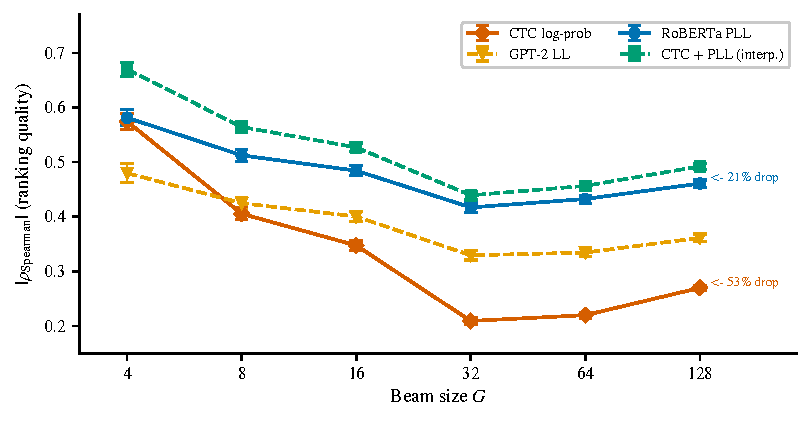
\includegraphics[width=\textwidth]{figures/fig6_spearman_divergence.pdf}
  \caption{Absolute Spearman $\rho$ between scorer and per-utterance WER vs beam size $G$ (error bars: 95\% CI). CTC log-probability degrades sharply (53\% drop, $G=4\to128$); RoBERTa PLL degrades gracefully (21\% drop). This divergence explains the MBR-vs-interpolation asymmetry in Fig.~\ref{fig:gscaling}.}
  \label{fig:spearman}
\end{figure*}

\textbf{The Spearman $\rho$ divergence.} Figure~\ref{fig:spearman} plots per-utterance Spearman $\rho$ for CTC log-prob
and RoBERTa PLL as a function of $G$. The divergence provides the mechanistic explanation for the
interpolation-MBR asymmetry, and its structure predicts the failure modes in §6.

At $G$=4, CTC $\rho$ ($-$0.574) and PLL $\rho$ ($-$0.581) were nearly equal: both scorers ranked small
candidate sets with comparable effectiveness. As $G$ grew, the two trajectories separated sharply.
Table~\ref{tab:spearman} gives the full progression from the beam-size scaling experiment.

\begin{table}[h]
\centering
\caption{Ranking divergence: per-utterance Spearman $\rho$ by beam size, CTC log-prob vs
RoBERTa PLL.}
\label{tab:spearman}
\begin{tabular}{rrrr}
\hline
$G$ & CTC $\rho$ & PLL $\rho$ & Gap ($|\Delta\rho|$) \\
\hline
4 & $-$0.574 & $-$0.581 & 0.007 \\
8 & $-$0.406 & $-$0.513 & 0.107 \\
16 & $-$0.347 & $-$0.484 & 0.137 \\
32 & $-$0.209 & $-$0.417 & 0.208 \\
64 & $-$0.220 & $-$0.433 & 0.213 \\
128 & $-$0.270 & $-$0.461 & 0.191 \\
\hline
\end{tabular}
\end{table}

CTC $\rho$ fell from $-$0.574 at $G$=4 to $-$0.209 at $G$=32 — a 64\% degradation — then partially
recovered to $-$0.270 at $G$=128. PLL $\rho$ fell from $-$0.581 to $-$0.461 across the same range, a 21\%
degradation. The divergence between the two trajectories is the key quantity.

CTC's degradation likely reflects blank-path proliferation specific to the lattice sampling process. Larger N-best lists
contain more near-duplicate candidates: lattice paths that differ only in blank placement but emit
the same token sequence. CTC assigns different log-probabilities to these paths because blank
insertion affects the path score, but the differences among near-duplicate paths are small and
acoustically uninformative. As $G$ grows, near-duplicate paths proliferate and dominate the
per-utterance ranking task; CTC's $\rho$ is dragged down by noise in the blank-position sub-ranking.
PLL scores the emitted text, ignoring blank placement entirely. Near-duplicate paths produce the same
text and receive the same PLL score; PLL is structurally invariant to the duplication that damages
CTC. PLL $\rho$ therefore declines gracefully rather than sharply.

The optimal interpolation weight $\alpha$ shifted from 0.7 (at $G$=4, 8, 16) to 0.8 (at $G \geq 32$),
reflecting the same effect: with more candidates, each individual PLL score carries a weaker signal
relative to the CTC anchor, and the optimal blend leans more on CTC. Even at the adjusted $\alpha$,
linear interpolation is confined to picking from a near-duplicate-cluttered list. MBR sidesteps this
by aggregating all $G$ PLL-weighted votes. Near-duplicate paths cast correlated votes in the CER sum
and their accumulated evidence is effectively denoised. The MBR solution is therefore more stable as
$G$ grows, independent of the per-candidate scoring noise.

This divergence explains why MBR first reached significance at $G$=8 while interpolation was already
near its ceiling at the same point. It also predicts the cross-condition failures examined in §6. In
VoxPopuli, 91.5\% of utterances have no candidate better than greedy; the candidate set has zero
recoverable diversity. The MBR consensus has no coherent signal to aggregate regardless of $G$. Under
MUSAN noise at 0 dB, CTC cannot generate phonetically distinct hypotheses and the oracle gap
collapses; again, candidate diversity is the prerequisite that is missing. The $\rho$ divergence
characterises a general principle: when candidate sets lack recoverable diversity, consensus-based
selection cannot outperform argmax any more than argmax can outperform greedy.

Table~\ref{tab:marginal_gain} shows marginal WER gain per $G$-doubling.
MBR-CER+PLL exhibits diminishing returns from $G=8$ through $G=64$
($-0.312$\,pp at the first doubling, $-0.063$\,pp at $G=32 \to 64$),
with a partial recovery at $G=64 \to 128$ ($-0.116$\,pp). Oracle WER
continues to improve at $0.18$--$0.42$\,pp per doubling, confirming that
the MBR ceiling is set by selection precision rather than candidate
coverage. Linear interpolation gains are negligible beyond $G=8$, consistent
with the argmax saturation described above.

\begin{table}[ht]
\caption{Marginal WER gain (pp) per $G$-doubling on dev-other.}
\label{tab:marginal_gain}
\centering
\small
\begin{tabular}{lccc}
\toprule
$G$ transition & MBR $\Delta$ & Oracle $\Delta$ & Interp.\ $\Delta$ \\
\midrule
$4 \to 8$     & $-0.312$ & $-0.404$ & $-0.124$ \\
$8 \to 16$    & $-0.096$ & $-0.418$ & $-0.001$ \\
$16 \to 32$   & $-0.080$ & $-0.309$ & $+0.006$ \\
$32 \to 64$   & $-0.063$ & $-0.207$ & $-0.002$ \\
$64 \to 128$  & $-0.116$ & $-0.183$ & $+0.006$ \\
\bottomrule
\end{tabular}
\end{table}

Further gains should come from better posterior estimation rather than larger candidate sets: each doubling of $G$ above 32 yielded approximately 0.07--0.08 pp of WER reduction for MBR, and a better-calibrated external LM would improve the PLL $\rho$ baseline at every $G$ level, amplifying the consensus effect.



\subsection{Temperature Calibration}

The temperature $\tau$ in the MBR posterior $w_j \propto \exp(\text{PLL}_j / \tau)$ controls the
sharpness of the language model prior over candidates. A temperature sweep covered
$\tau \in \{5, 6, 7, 8, 9, 10, 11, 12, 15, 20, 30, 50\}$ on the $G$=128 N-best with $B$=10\,000
paired bootstrap at each point. The sweep reveals two structural features in the
$\tau$ response: a phase transition below $\tau$=6 and a stable region above it.

At $\tau$=5, WER is 6.000\% ($\Delta$=$-$0.022 pp, $p$=0.383): not statistically significant. At
$\tau$=6, WER is 5.694\% ($\Delta$=$-$0.328 pp, $p$<0.0001). The step change of 0.306 pp in one
integer increment — accompanied by a transition from non-significance to $p$<0.0001 — is the sharpest
discontinuity in the entire sweep. The $\tau$=6 value was added to the sweep specifically to confirm
this boundary after the $\tau$=5-to-$\tau$=7 gap was observed. The transition is reproducible: it
marks the point where enough probability mass distributes across multiple candidates for the CER
consensus sum to discriminate among them. Below this threshold, the PLL posterior is peaked enough
that MBR approaches an argmax over PLL scores, and the posterior shape degenerates.

Above $\tau$=6, WER continues to improve through $\tau$=9 (WER 5.506\%, the statistical optimum),
then rises gradually. The region $\tau \in [8, 11]$ spans WER values within 0.04 pp of the optimum;
$\tau$=10 (5.529\%) is 0.024 pp above $\tau$=9. Beyond $\tau$=12, WER increases monotonically but
all points remain highly significant: at $\tau$=50, WER is 5.820\% ($p$<0.0001, $\Delta$=$-$0.202 pp).
Very high temperatures distribute mass nearly uniformly across all candidates, discarding the PLL
ranking information and approaching the self-consistency (uniform-weight MBR) result at $\tau \to
\infty$. The slow decay beyond $\tau$=12 reflects the gradual erasure of linguistic preference in the
posterior.

\begin{figure}[htbp]
  \centering
  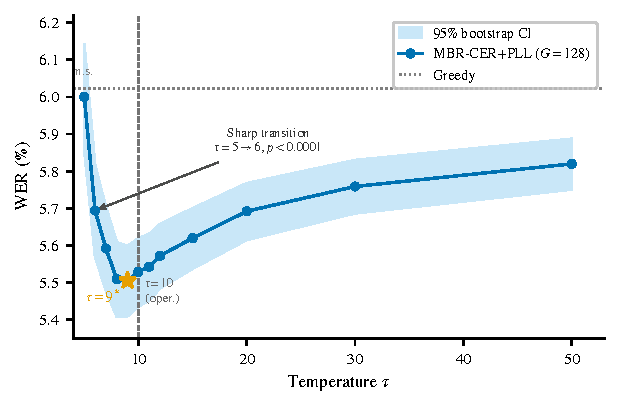
\includegraphics[width=\columnwidth]{figures/fig5_tau_sweep.pdf}
  \caption{WER as a function of temperature $\tau$ at $G=128$ (shaded: 95\% bootstrap CI for delta vs greedy). Sharp transition between $\tau=5$ (n.s., $p=0.38$) and $\tau=6$ ($\Delta=-0.328$\,pp, $p<0.0001$). WER is flat from $\tau=6$ to $\tau\approx15$ then degrades. Star: optimum $\tau=9$ (5.506\%); dashed: operational $\tau=10$ (5.529\%).}
  \label{fig:tau}
\end{figure}

Figure~\ref{fig:tau} plots WER as a function of $\tau$, with the non-significant region ($\tau$=5) and the
near-optimal plateau ($\tau \in [8, 11]$) identified. All experiments outside this temperature sweep use
$\tau$=10. The statistical optimum is $\tau$=9, and the 0.024 pp difference from $\tau$=10 is well
within the bootstrap 95\% CI for both. The flat region around the optimum guarantees that modest
$\tau$ misspecification does not materially change the outcome. No held-out tuning is required to
achieve near-optimal performance with this recipe.

The temperature $\tau$=10 was selected on the dev-other development set. The test-other evaluation
reported in §6.1 uses this value without any further adjustment, making test-other the
uncontaminated held-out evaluation of the final recipe. The gain on test-other ($-$0.535 pp) exceeds
the dev-other gain ($-$0.493 pp), confirming that the dev-other selection did not inflate the
test-other result.

\paragraph{Recipe summary.}
Table~\ref{tab:recipe} consolidates the complete decoding recipe for reference.

\begin{table}[h]
\centering
\small
\caption{Complete MBR-CER+PLL decoding recipe (all parameters fixed at dev-other selection).}
\label{tab:recipe}
\begin{tabular}{ll}
\hline
Parameter & Value \\
\hline
Beam size $G$ & 128 \\
Temperature $\tau$ & 10 \\
Loss function & CER (character error rate) \\
Posterior LM & RoBERTa-base \cite{liu2019roberta} \\
Posterior weights & $w_j \propto \exp(\mathrm{PLL}(y_j) / \tau)$ \\
Lattice sampling scale & \texttt{nbest\_scale}~=~1.0 \\
\hline
\end{tabular}
\end{table}

The posterior uses PLL scores only (no CTC component); the CTC model is used solely for candidate generation. In the notation of Equation~(11), the operational recipe sets the CTC exponent $\tau \to 0$ (suppressing the acoustic posterior component entirely) and $\alpha = 1/\tau_\text{PLL} = 1/10 = 0.1$, where $\tau_\text{PLL} = 10$ is the PLL temperature in the recipe's posterior weights $w_j \propto \exp(\text{PLL}(y_j)/\tau_\text{PLL})$. The recipe requires no modification to the acoustic model and no target-domain tuning.



All eleven CTC-internal methods fail at $G$=16. The Spearman $\rho$ divergence between CTC and RoBERTa PLL, established in §5.3, explains both why MBR continues improving with beam size while interpolation plateaus and why the recipe breaks down under the coverage conditions examined in §6.




